% Created 2022-06-08 Wed 11:26
% Intended LaTeX compiler: xelatex
\documentclass[11pt]{article}
\usepackage{graphicx}
\usepackage{longtable}
\usepackage{wrapfig}
\usepackage{rotating}
\usepackage[normalem]{ulem}
\usepackage{amsmath}
\usepackage{amssymb}
\usepackage{capt-of}
\usepackage{hyperref}
\usepackage{pdfpages}
\usepackage{graphicx}
\usepackage{amsmath}
\usepackage{mathtools}
\usepackage{amsfonts}
\usepackage{float}
\usepackage{array}
\usepackage{helvet}
\usepackage{color}
\definecolor{myblue}{rgb}{.8, .8, 1}
\usepackage{empheq}
\usepackage{tkz-euclide}
\usepackage{caption}

 \usepackage[margin=0.8in]{geometry}
\usepackage{pgfplots}
\pgfplotsset{compat=newest, ticks=none}

\newlength\mytemplen
\newsavebox\mytempbox

\makeatletter
\newcommand\mybluebox{%
    \@ifnextchar[%]
       {\@mybluebox}%
       {\@mybluebox[0pt]}}

\def\@mybluebox[#1]{%
    \@ifnextchar[%]
       {\@@mybluebox[#1]}%
       {\@@mybluebox[#1][0pt]}}

\def\@@mybluebox[#1][#2]#3{
    \sbox\mytempbox{#3}%
    \mytemplen\ht\mytempbox
    \advance\mytemplen #1\relax
    \ht\mytempbox\mytemplen
    \mytemplen\dp\mytempbox
    \advance\mytemplen #2\relax
    \dp\mytempbox\mytemplen
    \colorbox{myblue}{\hspace{1em}\usebox{\mytempbox}\hspace{1em}}}

\makeatother

\newcommand*\widefbox[1]{\fbox{\hspace{2em}#1\hspace{2em}}}


\newenvironment{amatrix}[1]{%
  \left(\begin{array}{@{}*{#1}{c}|c@{}}
}{%
  \end{array}\right)
}
\newcommand{\ro}[1]{%
  \xrightarrow{\mathmakebox[\rowidth]{#1}}%
}

\newlength{\rowidth}% row operation width
\AtBeginDocument{\setlength{\rowidth}{4em}}


\usepackage[thmmarks,  thref, amsmath]{ntheorem}

\theoremstyle{plain}
\newtheorem{thm}{Theorem}

\theoremheaderfont{\itshape}
\theorembodyfont{\upshape}
\newtheorem{case}{Case}

\theoremstyle{nonumberplain}
\theoremheaderfont{\scshape}
\theorembodyfont{\upshape}
\theoremsymbol{\scshape Q. E. D.}% or\ensuremath{ _{\Box}}, also add \usepackage{amssymb}
% or O. E. \ensuremath{\Delta} % for Euclid's  ὅπερ ἔδει δεῖξαι
\theorempostwork{\setcounter{case}{0}}
\newtheorem{proof}{Proof}

%%% Local Variables:
%%% mode: latex
%%% TeX-master: "Assignment"
%%% End:

\setcounter{secnumdepth}{2}
\author{Abhaas Goyal \& Kaushiki Jadhav}
\date{\today}
\title{ENGN4213 Report}
\hypersetup{
 pdfauthor={Abhaas Goyal \& Kaushiki Jadhav},
 pdftitle={ENGN4213 Report},
 pdfkeywords={},
 pdfsubject={},
 pdfcreator={Emacs 28.1 (Org mode 9.6)}, 
 pdflang={English}}
\begin{document}

\maketitle
\setlength\parindent{0pt}


\section{Hardware Connections}
\label{sec:orge2f46f7}
Here in this project, we have used different hardware tools and connected to each other for taking input data, processing data, and showing output data which are explained below:

\begin{figure}[H]
    \centering
    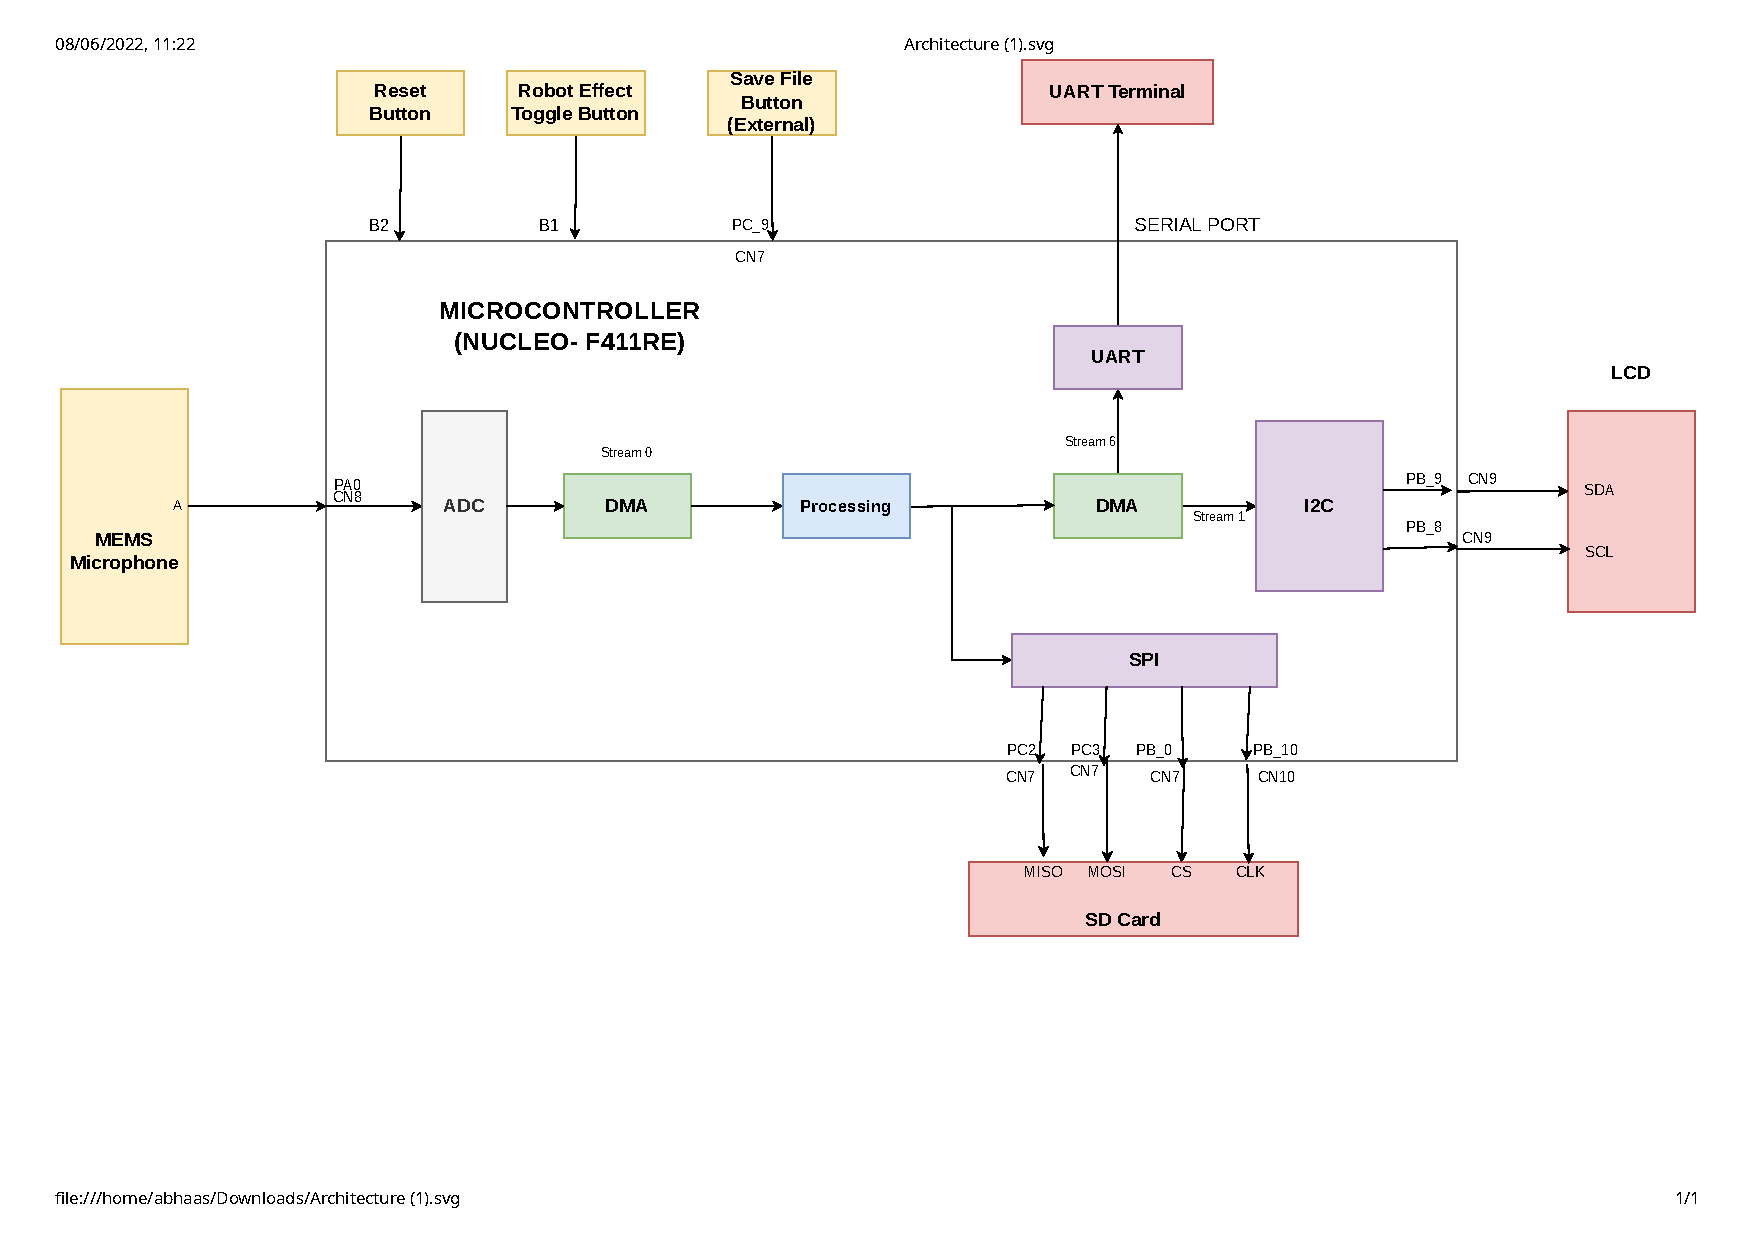
\includegraphics[width=1\textwidth, trim={0cm 5cm 0cm 1cm}, clip]{Architecture.pdf}
    \caption{Overall Architecture}
    \end{figure}

\subsection{Microphone}
\label{sec:org609154e}

\begin{itemize}
\item Protocols used => \textbf{ADC + DMA}
\end{itemize}

We use a Female MEMS microphone module (SEN0487 - Manufacturer DFROBOT [MIC Module (V1.0) [21BLg] 65Z5]) having a gain of 66. This module can be used at both 3.3V/5V (downscaling of 5V -> 3.3V is present in the module itself). For the purposes of long time safety, we use the 3.3V version. We can get an acoustic waveform by ADC sampling from the initial analog input audio signal from the microphone. When there is no input signal then its output voltage is around 0.66*VCC.

Here microphone is used as an input device for the project which gives acoustic waves signals to ADC for further process of the project. The microphone’s A pin is connected to the IN0 function of the ADC peripheral which is the A0/PA0 (since our initial input is analog so we need to have an ADC converter - given through this port).

To save unneccessary clock cycles to saving it to contiguous memory locations in the buffer and doing the fixed process of resolution again, this process is taken care of by the DMA. We use a circular buffer of a fixed size and the input is taken as half words (since we are using 12 bits for resolution - the maximum available in this module for maximal precision)


\subsection{SD Card}
\label{sec:orgfa59839}

\begin{itemize}
\item Communication Protocol => \textbf{SPI}
\end{itemize}

The output data of the project is saved on an SD card. For connecting SD card with a microcontroller SD card adapter is used and which is connected to the SPI serial communication peripheral of the microcontroller. The used voltage is 5V for efficient usage of SD Card.

\subsection{LCD}
\label{sec:org353e4a6}

\begin{itemize}
\item Communication Protocol => \textbf{I2C}
\end{itemize}

We use a \texttt{lcd-1602a-qapass} LCD module with soldered pins and inbuilt I2C module for communication
LCD is connected to the I2C serial communication peripheral for showing a dominant frequency of the audio signal.

\subsection{Push button}
\label{sec:org9b8f643}

\begin{itemize}
\item Communication Protocol => \textbf{General Purpose Input}
\end{itemize}

for saving data files in sd card.

\section{Implementation}
\label{sec:orge4b4b0b}
\subsection{Design Flow}
\label{sec:org4a0a02e}
\begin{enumerate}
\item Microphone sends data to Microcontroller at 4000Hz
\item Through ADC and DMA, store store the data in input buffer
\item Pass input data to a high pass filter to remove signals which have a frequency below 200 Hz.
\item If robot effect is on, then enable privacy mode. Processing of privacy mode is done by the robot effect (implemented by fast delay) and then a different high pass filter is used (according to the person's voice) to remove low-frequency signals.
\item The output data is shown on UART.
\item The output data will pass to FFT and then the maximum dominant frequency will display on LCD.
\item All processed data will save on the SD card.
\item By using audio signal processing libraries on the PC (file provided in MATLAB), we can hear our desired output audio.
\end{enumerate}

\subsection{Data Flow in Buffers}
\label{sec:orgda4797a}
Since we are working on a large amount of continuous analog input data, where real-time processing needs to be implemented with constraints on the size of the buffer possible. Hence the frame based processing (block) is used to process the data. A 4 buffer ping-pong is used to processing a complete block of the sample, while the other half is being inputted.

\subsubsection*{Pong Buffers used in the project:}
\label{sec:org66eea40}

\begin{itemize}
\item \texttt{q15\_t in\_buf [INPUT\_BUF\_SIZE]} = Used to store data or samples that are captured from a microphone
\item \texttt{q15\_t out\_buf [OUTPUT\_BUF\_SIZE]} = Used to store data or samples after processing
\item \texttt{char out\_buf\_char [OUTPUT\_BUF\_CHAR\_SIZE]} = Used for sending data in a string via UART and saving file I/O
\end{itemize}

\subsubsection*{Pointers to buffer's are used to fill currently data in buffer at exact address:}
\label{sec:orgbbc408a}

\begin{itemize}
\item \texttt{q15\_t* in\_buf\_ptr} = Input buffer pointer
\item \texttt{q15\_t* out\_buf\_ptr} = Output buffer pointer
\item \texttt{char* out\_buf\_char\_ptr} = Output character buffer pointer
\end{itemize}

\subsubsection*{Size of buffers used in the project:}
\label{sec:org25d44eb}
\begin{itemize}
\item \texttt{FILTER\_TAP\_NUM 30} -> for implementing a high pass filter (originally, there were 29 tap values) are used that is filter coefficient values as per designed filter values. Since the number of taps needs to be even, I made the last tap have the value as 0
\item \texttt{INPUT\_PROCESS\_BUF\_SIZE 512} –> 512 samples will be processed in a single block. This was deemed optimal for maximal processing while signalling to display to UART and writing to a file
\item \texttt{INPUT\_BUF\_SIZE (INPUT\_PROCESS\_BUF\_SIZE * 2)} -> input buffer size has double the size of the input process buffer size (ping and pong of the buffer).
\item \texttt{OUTPUT\_PROCESS\_BUF\_SIZE = INPUT\_PROCESS\_BUF\_SIZE}
\item \texttt{OUTPUT\_BUF\_SIZE = INPUT\_BUF\_SIZE}
\item \texttt{OUTPUT\_PROCESS\_CHAR\_BUF\_SIZE (INPUT\_PROCESS\_BUF\_SIZE * 5)} -> This Output process character buffer has 5 times the size of the input process buffer size to use the processed data in a character form for (a) displaying in UART (consisting of 4 characters separated by \texttt{\textbackslash{}n} at a time) and (b) to save file SD card.
\item \texttt{OUTPUT\_BUF\_CHAR\_SIZE (OUTPUT\_PROCESS\_CHAR\_BUF\_SIZE * 2)} -> Maps to other part
\end{itemize}

\subsection{Reason to choose Q15}
\label{sec:org402e760}

The Q15 number has a integral range between \texttt{(-2\textasciicircum{}16)} and \texttt{(2\textasciicircum{}16 - 1)}, scaled up from (-1.0, 1.0) w.r.t. floating point numbers. Since the operations in this type are done between integral types which are much faster than their counterparts (floating point types), it makes it very convenient in DSP where real time processing has to be completed.

\subsection{Flow of data in buffers}
\label{sec:org658853b}

The input buffer size has a double size of the input process buffer size. The input data from ADC will store in the input buffer. When half input buffer will be full (we can call it a single block) then the flag \texttt{write\_file\_chunk\_flag} will generate and indicate that the input buffer is half full and will trigger the process function/event for that block. Then that half-full input buffer data will be used for processing. After processing is completed, that processed data will store in half of the output buffer. Then that integer data will store in the output character buffer in the form of a string that data will show on the UART.  Simultaneously, while processing the first block or half input buffer, the remaining half input buffer will store data via DMA, after completely full the input buffer then again flag \texttt{write\_file\_chunk\_flag} will generate and indicate the input buffer is full and again trigger the process function/event for remained data in half input buffer that is the second block. That processed data will store in the output buffer and again data will pass to the output char buffer from the output buffer for showing data on UART. After the flag is generated \texttt{write\_file\_chunk\_flag} ADC will start storing data in the input buffer via DMA peripheral. This process is continued in a circular manner. In this project we are working with a large amount of data hence DMA is working as the pipeline for storing data in buffers and also sending data to UART.

\begin{figure}[H]
    \centering
    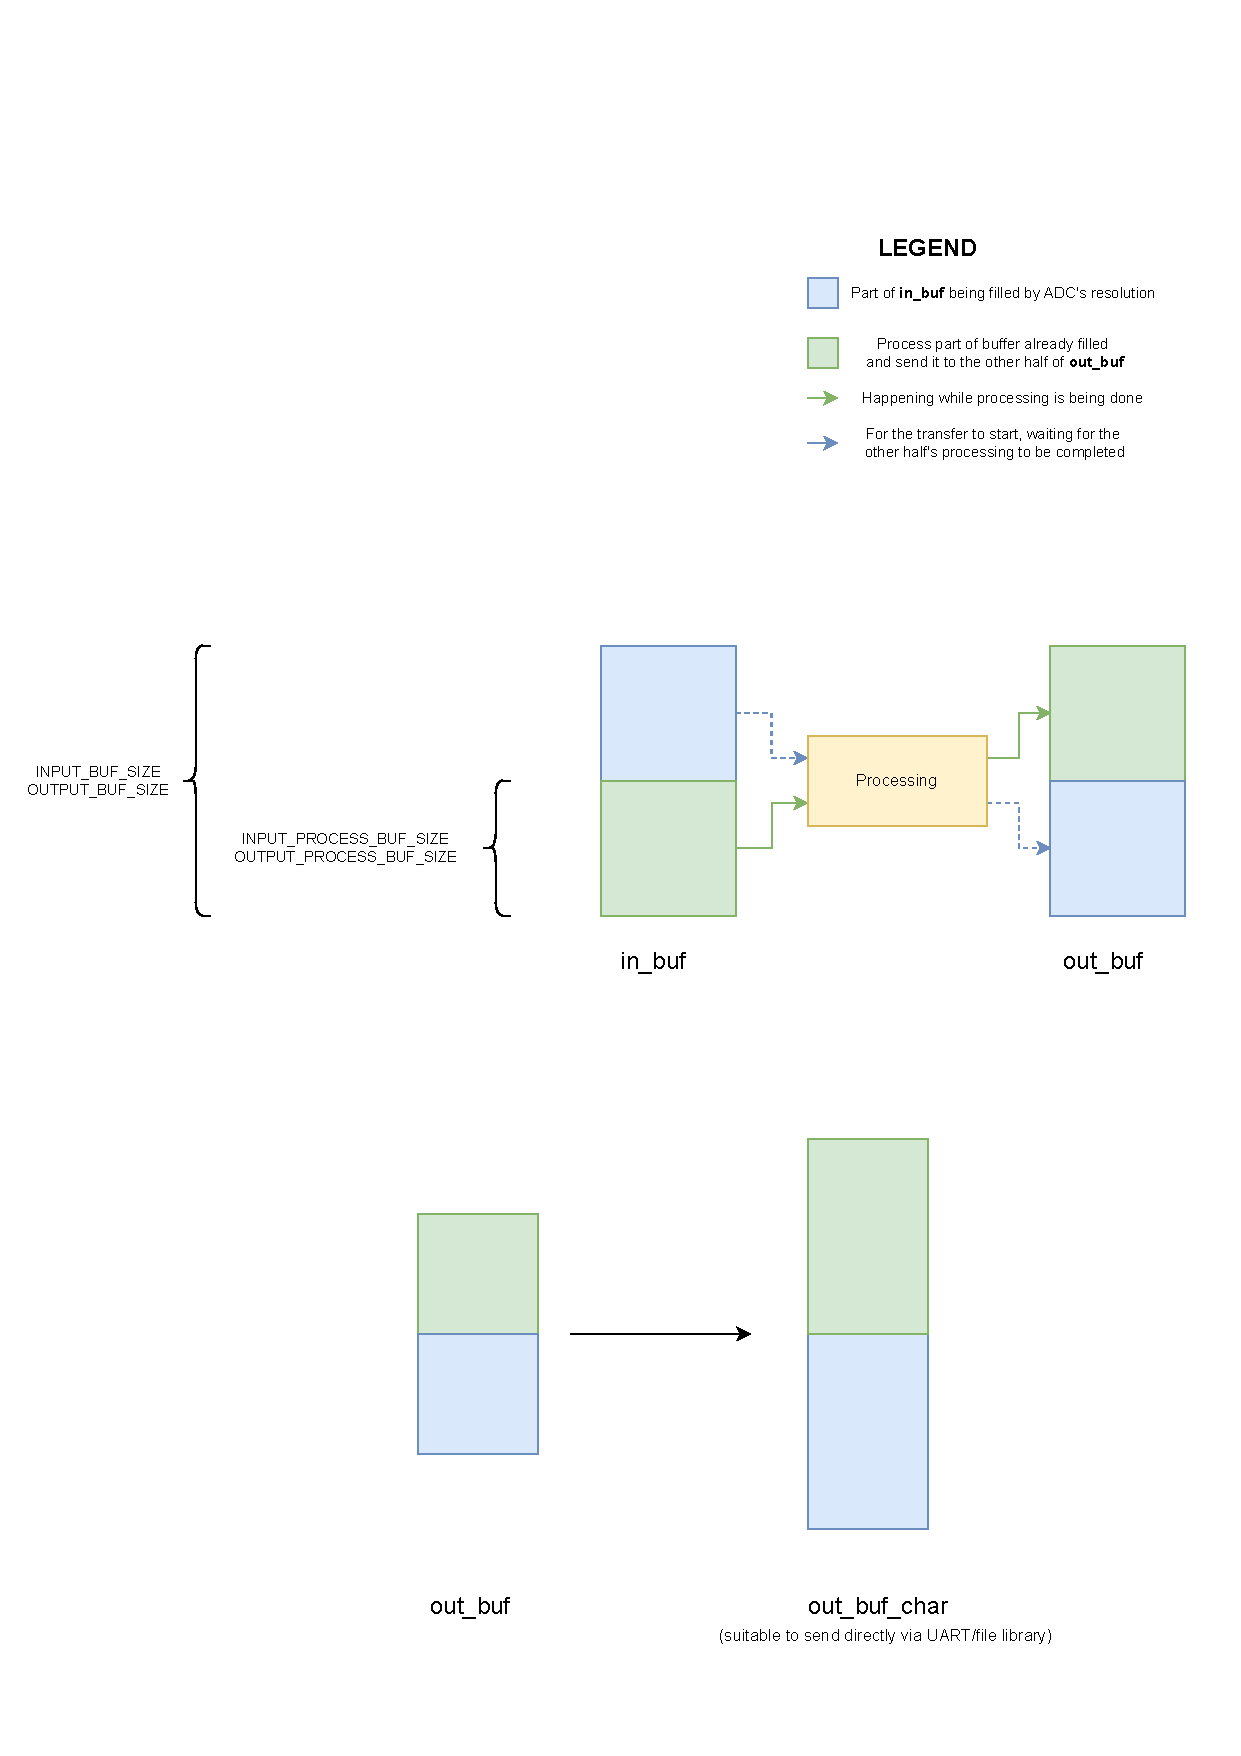
\includegraphics[width=1\textwidth, trim={0cm 1cm 0cm 4cm}, clip]{IO_Buffer_Structure.pdf}
    \caption{I/O Buffer Structure}
    \end{figure}

\subsection{Interrupts}
\label{sec:org86f3d13}

\begin{itemize}
\item Half full
\item Full full
\item robot effect
\end{itemize}

\subsection{Timers}
\label{sec:org88b2049}

\begin{itemize}
\item \texttt{TIM2} for the ADC's DMA to synchronize to input values and store them into the input buffer. It was chosen since the timer needed to be somewhat advanced with supported DMA and interrupts.
\item \texttt{TIM9} as the timebase source for RTOS. It was chosen because the timebase source needed to be simple enough for count reference.
\end{itemize}

\subsection{Input data / ADC}
\label{sec:org05730ed}


The microphone is connected to ADC peripheral to convert analog signals to digital signals. The microphone will send acoustic waveforms of input audio to ADC peripheral. ADC peripheral will convert that analog signal into digital data that digital data ADC stores input data in the input buffer via DMA peripheral.
For taking real-time input, the CPU clock is set to 100MHz, and to take ADC samples for the desired frequency ADC clock Prescaler is set to 25MHz i.e., PCLK divided 4 and resolutions to 12 bits (15 ADC clock cycles) which means will take values between 0 to 2\textsuperscript{12} bits. Hence ADC samples can be taken independently from the CPU clock. The \textbf{sampling frequency} is 4000Hz which means in 1 sec 4000 samples will take.  Also, connect DMA peripheral to the ADC1 peripheral to send a large amount of data from the peripheral to memory.  The microphone will send acoustic waveforms to ADC and will convert that analog signal into digital signals. That digital signals or sampling data will store in the input buffer for processing. Plotted that data in the form of a graph in MATLAB it is observed that the microphone is receiving a large amount of data which has different frequencies with the fluctuation in amplitude.

\section{Data processing}
\label{sec:orgb86537f}

\begin{figure}[H]
    \centering
    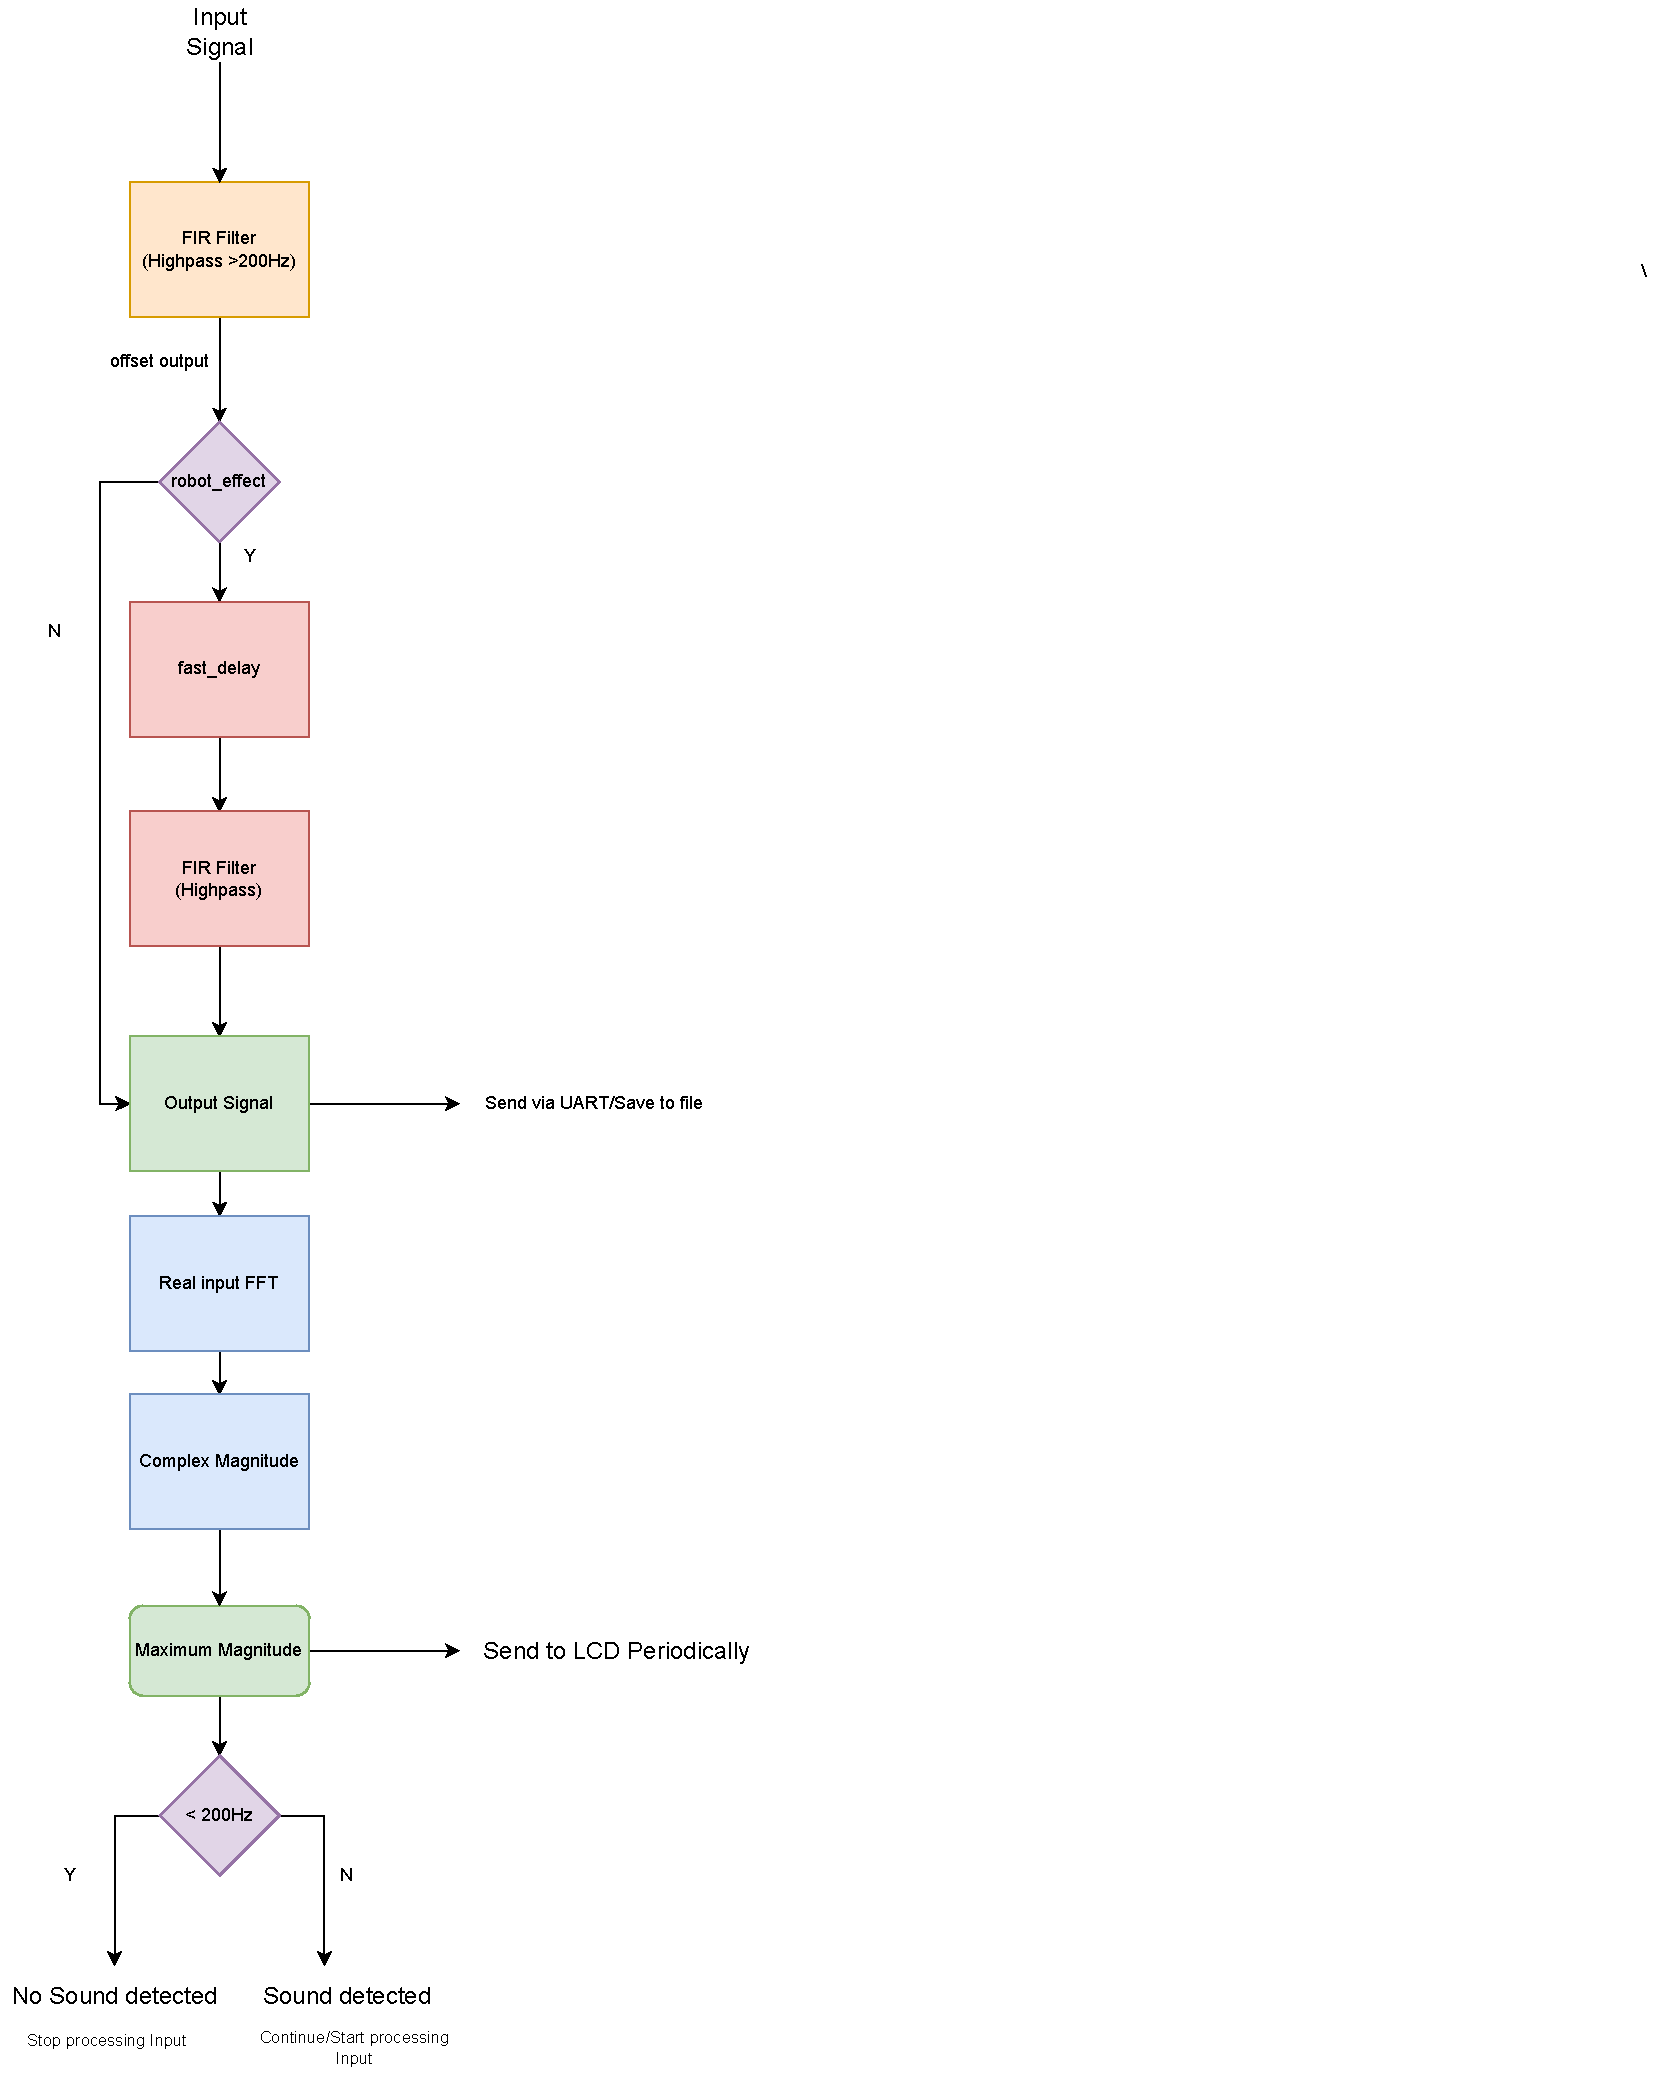
\includegraphics[width=0.45\textwidth, trim={0cm 0cm 15cm 0cm}, clip]{Processing.pdf}
    \caption{Processing}
    \end{figure}

\subsection{High pass filter}
\label{sec:org7e532f7}

A high pass filter is a filter that passes high-frequency signals and blocks, or impedes, low-frequency signals. A high pass filter is used to remove frequencies below 200Hz.
To implement a high pass filter on MCU, the CMSIS DSP software library is used. In particular arm\textsubscript{math.h} library and lib file are imported into the project which has functions of a high-pass filter.
FIR filter is designed by using \url{http://t-filter.appspot.com} this software, got the desired tap values that is filter coefficient values for implementing the high pass filter in the project. For designing set values according to project task requirements which are as follows.


\begin{table}[htbp]
\centering
\begin{tabular}{|c|c|c|c|c|c|c|c|c|c|c|c|c|c|c|c|c|}
\hline
from & to & gain & Ripple/Attenuation & Actual Ripple\\
\hline
0 Hz & 150 Hz & 0 & -20 dB & -20.08 dB\\
220 Hz & 2000 Hz & 1 & 5 dB & 4.14 dB\\
\hline
\end{tabular}
\caption{Highway Management Output Logic}

\end{table}


\begin{figure}[H]
    \centering
    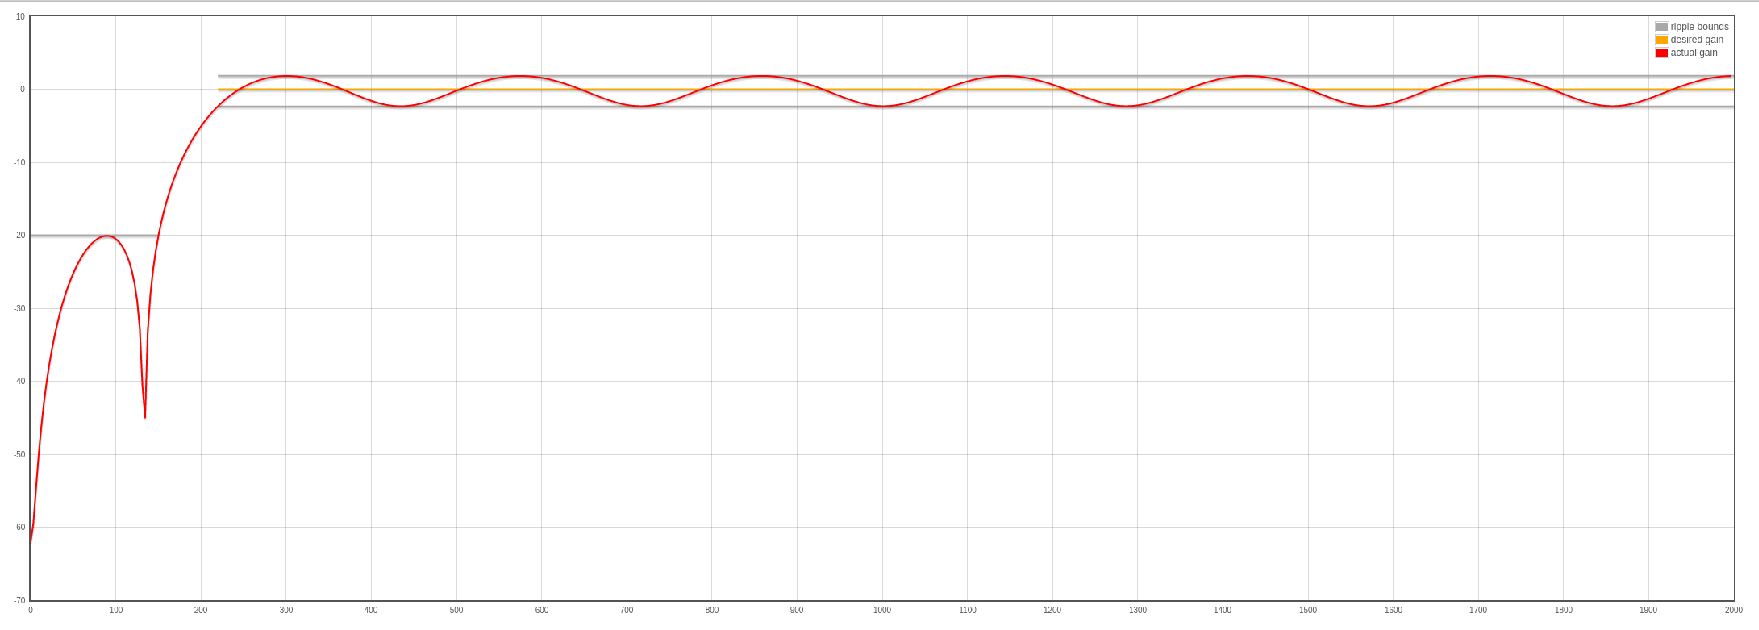
\includegraphics[width=1\textwidth, trim={0cm 0cm 0cm 0cm}, clip]{Filter.pdf}
    \caption{Designed Filter}
    \end{figure}


29 tap values that are filter coefficients are required for this designed high pass filter. The input process buffer has a size of 512 which means 512 samples will be processed in a single block.
When flag \texttt{write\_file\_chunk\_flag==1} is generated it will trigger the process function which means 512 samples are stored in the input process buffer.
For implementing a high-pass filter DSP library needs some internal FIR instance settings hence FIR instance declared \texttt{arm\_fir\_instance\_q15 fir\_settings} and also needs internal FIR states which have a size always equal to \texttt{INPUT\_PROCESS\_BUF\_SIZE + FILTER\_TAP\_NUM - 1}.
For processing DSP library has single line function that is:

\begin{verbatim}
arm_fir_q15(&fir_settings, in_buf_ptr, out_buf_ptr, INPUT_PROCESS_BUF_SIZE);
\end{verbatim}

Here, we passed the address for FIR instance setting, input buffer pointer for processing input data, and output buffer pointer to store processed output data in the output buffer. Output data will store in the output buffer for further process and data to display on UART.
Below 200Hz frequency will filter out and amplitude will be normalized. By using a high-pass filter.
After using a high pass filter, we have given an offset of 2000 to normalize amplitude. We implemented this calculation of negative values is difficult to do. for easy implementation of further processes.

\subsection{Robot effect}
\label{sec:org091cd0a}
For robot effect here fast delay implemented

\subsubsection*{Fast delay}
\label{sec:org41fadc2}
Here implemented fast delay. We took an average of 5 samples. Divided samples into chunks and take an average of the previous four samples and one current sample.  That averaged samples frequency reach at 9000 the again samples normalized again we put offset of -7000. and saved data into the input process buffer
\subsubsection*{High pass filter}
\label{sec:org05f91bd}
That data again passed to a high pass filter to remove low-frequency data. After passing again gave an offset of 2000 to normalize the amplitude of processed data.

\begin{figure}[H]
    \centering
    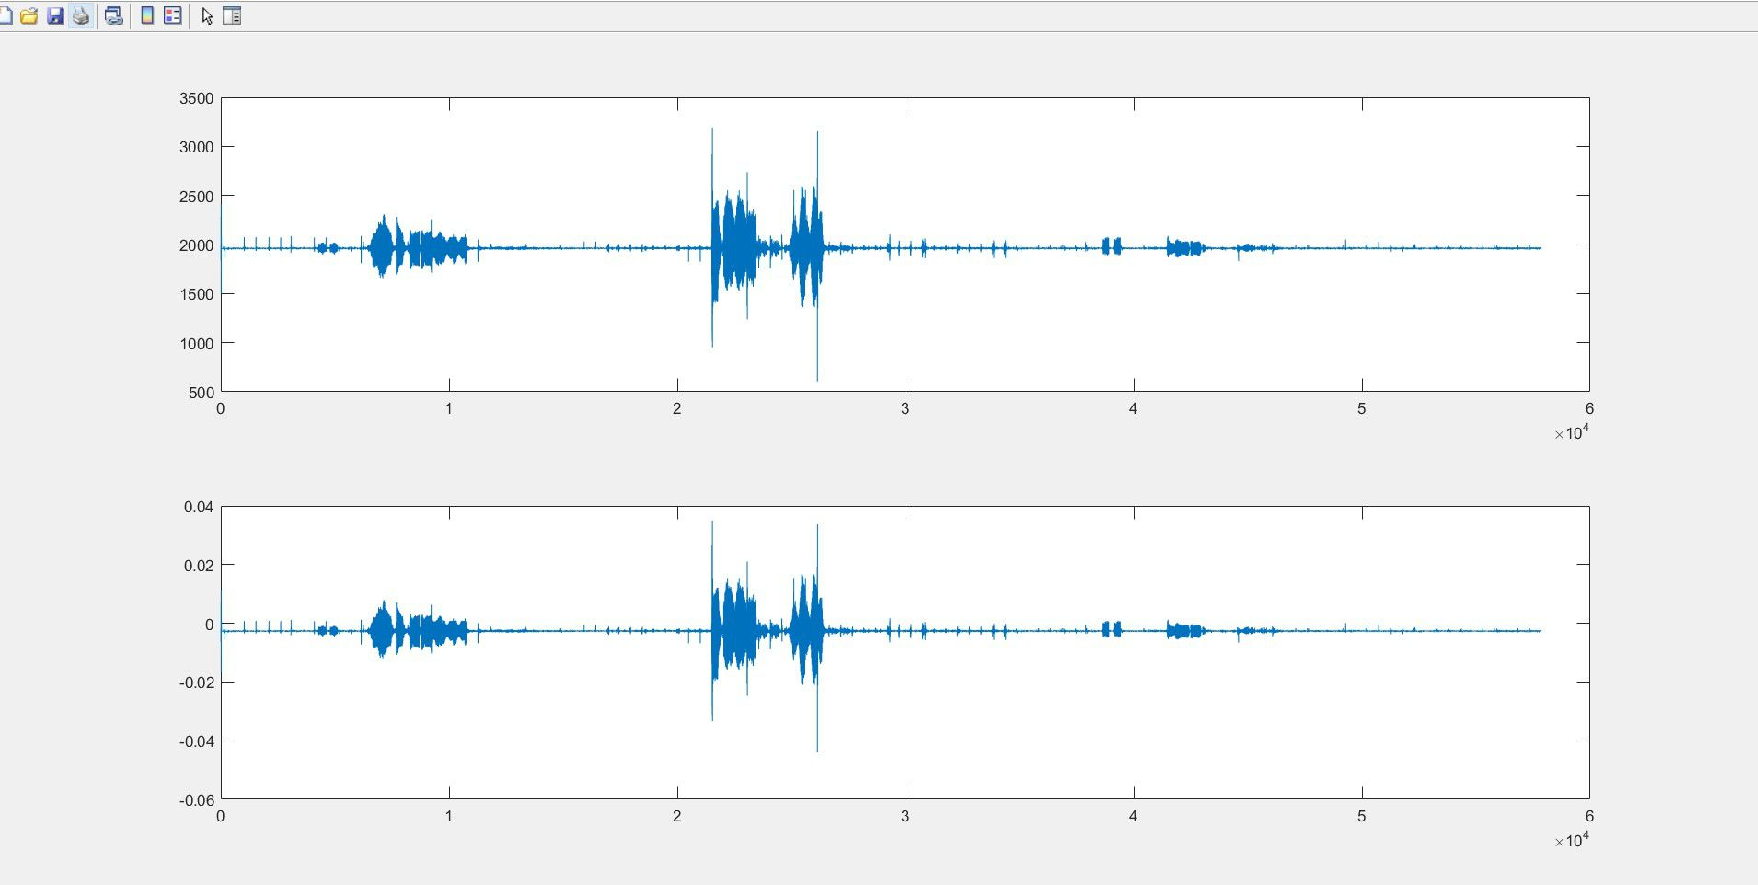
\includegraphics[width=1\textwidth, trim={0cm 0cm 0cm 0cm}, clip]{SD_Read.pdf}
    \caption{SD Card File Output Read}
    \end{figure}

\subsection{FFT}
\label{sec:org33bc954}

Data is copied in a separate bufffer for calculating FFT. Complex magnitude is taken and maximal of those is taken

The maximum value is printed every second

\subsection{Sound activity}
\label{sec:org0ff945c}

If maximum FFT Freq < 200Hz then no sound else sound


\section{Output data}
\label{sec:org88c9124}

\subsection{UART}
\label{sec:org0468f83}

When flag \texttt{write\_file\_chunk\_flag ==1} then sample block will go to processing. When the process will complete, the processed data will store in the output buffer \texttt{out\_char\_buf}. To display processed data via serial communication on PC that stored data will send to UART in string form. A UART Terminal Client is used to display data on pc via serial communication (For example Hercules / CoolTern). Baud rate is set to 230400 baud.

\subsubsection*{Graph}
\label{sec:org1e8b54f}
See code on appendix A

\subsection{SD Card}
\label{sec:org03ff77c}


\subsubsection*{Mount}
\label{sec:orge3faf3d}
First will mount the SD card and check for it's successful mounting. If there is an error with the file system / other problems in mounting then the appropriate error message will be shown. For debugging purposes, we also check for the free space and calculate the total size of the SD card using the pointer and the size and free space of the SD. All the results are also displayed in UART.
\subsubsection*{Write}
\label{sec:orgcb88853}

After processing the first block of sample data, the processed data will store in the output buffer[output\textsubscript{char}\textsubscript{buf}] then flag [write\textsubscript{file}\textsubscript{chunk}\textsubscript{flag}==2] will generate and will trigger the SD card saving function and also check whether another half input buffer has been filled after processing the first block. If there is a current file existed then the current file opens and filling data in the SD card will start and will save data in the current file in the SD card in string form. When writing will be done then the current file will close. If there is no current file then a new file will generate and open that file for writing the data.
To save multiple files on an SD card, the names of files should be different for different data hence we updated file names as data updated. To save a new file with a different name on an SD card the name of the file will change with the current file number changes.
Here we have used a switch to save files which means that if press switch then the current file will close and the new file will open and data will store in the new file.


\subsection{LCD}
\label{sec:org87487ab}

If the frequency of input data is below 200Hz then no sound is detected message will show on LCD and if input data frequency is above 200Hz then maximum frequency and robot effect is on or off will show on the LCD.

Max = 0000 and R 0 if the robot effect is off and R 1 if the robot effect is on.

\section{Appendix}
\label{sec:org36b9c13}
\subsection{Graph plot}
\label{sec:org9c7e5d3}

\begin{verbatim}
import serial
from time import sleep
import matplotlib.pyplot as plt
import numpy as np

robot_effect = 0
default_mean_ampl = 4000 if robot_effect else 2000
ylim_arg = [3500, 4500] if robot_effect else [1500, 2500]


ser = serial.Serial ("/dev/ttyACM0", 230400)    #Open port with baud rate
while True:
    received_data = ser.read()              #read serial port
    sleep(0.2)
    data_left = ser.inWaiting()             #check for remaining byte
    received_data += ser.read(data_left)
    received_data = received_data.decode("utf-8")

    received_data = received_data.split("\n")
    received_data = list(map(lambda x: int(x) if x != '' else default_mean_ampl, received_data))
    received_data = list(filter(lambda x: x > 0 and x < 10000, received_data))
    print(received_data)

    xpoints = np.arange(len(received_data))
    plt.clf()
    plt.plot(xpoints, received_data)
    plt.ylim(ylim_arg)
    plt.pause(0.05)
\end{verbatim}
\end{document}
